\documentclass{article}
\usepackage[utf8]{inputenc}
\usepackage{graphicx}
\usepackage{siunitx}
\usepackage{color}
\usepackage{tikz}

\title{Test}
\author{Paul Große-Bley}
\date{April 2018}

\begin{document}

\begin{figure}
	% GNUPLOT: LaTeX picture with Postscript
\begingroup
  % Encoding inside the plot.  In the header of your document, this encoding
  % should to defined, e.g., by using
  % \usepackage[latin1,<other encodings>]{inputenc}
  \inputencoding{latin1}%
  \makeatletter
  \providecommand\color[2][]{%
    \GenericError{(gnuplot) \space\space\space\@spaces}{%
      Package color not loaded in conjunction with
      terminal option `colourtext'%
    }{See the gnuplot documentation for explanation.%
    }{Either use 'blacktext' in gnuplot or load the package
      color.sty in LaTeX.}%
    \renewcommand\color[2][]{}%
  }%
  \providecommand\includegraphics[2][]{%
    \GenericError{(gnuplot) \space\space\space\@spaces}{%
      Package graphicx or graphics not loaded%
    }{See the gnuplot documentation for explanation.%
    }{The gnuplot epslatex terminal needs graphicx.sty or graphics.sty.}%
    \renewcommand\includegraphics[2][]{}%
  }%
  \providecommand\rotatebox[2]{#2}%
  \@ifundefined{ifGPcolor}{%
    \newif\ifGPcolor
    \GPcolortrue
  }{}%
  \@ifundefined{ifGPblacktext}{%
    \newif\ifGPblacktext
    \GPblacktextfalse
  }{}%
  % define a \g@addto@macro without @ in the name:
  \let\gplgaddtomacro\g@addto@macro
  % define empty templates for all commands taking text:
  \gdef\gplbacktext{}%
  \gdef\gplfronttext{}%
  \makeatother
  \ifGPblacktext
    % no textcolor at all
    \def\colorrgb#1{}%
    \def\colorgray#1{}%
  \else
    % gray or color?
    \ifGPcolor
      \def\colorrgb#1{\color[rgb]{#1}}%
      \def\colorgray#1{\color[gray]{#1}}%
      \expandafter\def\csname LTw\endcsname{\color{white}}%
      \expandafter\def\csname LTb\endcsname{\color{black}}%
      \expandafter\def\csname LTa\endcsname{\color{black}}%
      \expandafter\def\csname LT0\endcsname{\color[rgb]{1,0,0}}%
      \expandafter\def\csname LT1\endcsname{\color[rgb]{0,1,0}}%
      \expandafter\def\csname LT2\endcsname{\color[rgb]{0,0,1}}%
      \expandafter\def\csname LT3\endcsname{\color[rgb]{1,0,1}}%
      \expandafter\def\csname LT4\endcsname{\color[rgb]{0,1,1}}%
      \expandafter\def\csname LT5\endcsname{\color[rgb]{1,1,0}}%
      \expandafter\def\csname LT6\endcsname{\color[rgb]{0,0,0}}%
      \expandafter\def\csname LT7\endcsname{\color[rgb]{1,0.3,0}}%
      \expandafter\def\csname LT8\endcsname{\color[rgb]{0.5,0.5,0.5}}%
    \else
      % gray
      \def\colorrgb#1{\color{black}}%
      \def\colorgray#1{\color[gray]{#1}}%
      \expandafter\def\csname LTw\endcsname{\color{white}}%
      \expandafter\def\csname LTb\endcsname{\color{black}}%
      \expandafter\def\csname LTa\endcsname{\color{black}}%
      \expandafter\def\csname LT0\endcsname{\color{black}}%
      \expandafter\def\csname LT1\endcsname{\color{black}}%
      \expandafter\def\csname LT2\endcsname{\color{black}}%
      \expandafter\def\csname LT3\endcsname{\color{black}}%
      \expandafter\def\csname LT4\endcsname{\color{black}}%
      \expandafter\def\csname LT5\endcsname{\color{black}}%
      \expandafter\def\csname LT6\endcsname{\color{black}}%
      \expandafter\def\csname LT7\endcsname{\color{black}}%
      \expandafter\def\csname LT8\endcsname{\color{black}}%
    \fi
  \fi
    \setlength{\unitlength}{0.0500bp}%
    \ifx\gptboxheight\undefined%
      \newlength{\gptboxheight}%
      \newlength{\gptboxwidth}%
      \newsavebox{\gptboxtext}%
    \fi%
    \setlength{\fboxrule}{0.5pt}%
    \setlength{\fboxsep}{1pt}%
\begin{picture}(8502.00,5102.00)%
    \gplgaddtomacro\gplbacktext{%
      \csname LTb\endcsname%%
      \put(814,704){\makebox(0,0)[r]{\strut{}$1.2$}}%
      \put(814,1168){\makebox(0,0)[r]{\strut{}$1.3$}}%
      \put(814,1632){\makebox(0,0)[r]{\strut{}$1.4$}}%
      \put(814,2096){\makebox(0,0)[r]{\strut{}$1.5$}}%
      \put(814,2560){\makebox(0,0)[r]{\strut{}$1.6$}}%
      \put(814,3025){\makebox(0,0)[r]{\strut{}$1.7$}}%
      \put(814,3489){\makebox(0,0)[r]{\strut{}$1.8$}}%
      \put(814,3953){\makebox(0,0)[r]{\strut{}$1.9$}}%
      \put(814,4417){\makebox(0,0)[r]{\strut{}$2$}}%
      \put(814,4881){\makebox(0,0)[r]{\strut{}$2.1$}}%
      \put(946,484){\makebox(0,0){\strut{}$-0.3$}}%
      \put(1841,484){\makebox(0,0){\strut{}$-0.2$}}%
      \put(2736,484){\makebox(0,0){\strut{}$-0.1$}}%
      \put(3631,484){\makebox(0,0){\strut{}$0$}}%
      \put(4526,484){\makebox(0,0){\strut{}$0.1$}}%
      \put(5420,484){\makebox(0,0){\strut{}$0.2$}}%
      \put(6315,484){\makebox(0,0){\strut{}$0.3$}}%
      \put(7210,484){\makebox(0,0){\strut{}$0.4$}}%
      \put(8105,484){\makebox(0,0){\strut{}$0.5$}}%
    }%
    \gplgaddtomacro\gplfronttext{%
      \csname LTb\endcsname%%
      \put(198,2792){\rotatebox{-270}{\makebox(0,0){\strut{}$\frac{\langle L^4 \rangle}{\langle L^2 \rangle^2}$}}}%
      \put(4525,154){\makebox(0,0){\strut{}$\frac{\beta - \beta_c}{\beta_c}N_\sigma^{1/\nu}$}}%
      \csname LTb\endcsname%%
      \put(7118,4708){\makebox(0,0)[r]{\strut{}$N_\sigma =\  8$}}%
      \csname LTb\endcsname%%
      \put(7118,4488){\makebox(0,0)[r]{\strut{}$N_\sigma =\  9$}}%
      \csname LTb\endcsname%%
      \put(7118,4268){\makebox(0,0)[r]{\strut{}$N_\sigma = 10$}}%
      \csname LTb\endcsname%%
      \put(7118,4048){\makebox(0,0)[r]{\strut{}$N_\sigma = 11$}}%
      \csname LTb\endcsname%%
      \put(7118,3828){\makebox(0,0)[r]{\strut{}$N_\sigma = 12$}}%
      \csname LTb\endcsname%%
      \put(7118,3608){\makebox(0,0)[r]{\strut{}$N_\sigma = 13$}}%
      \csname LTb\endcsname%%
      \put(7118,3388){\makebox(0,0)[r]{\strut{}$N_\sigma = 14$}}%
      \csname LTb\endcsname%%
      \put(7118,3168){\makebox(0,0)[r]{\strut{}$N_\sigma = 15$}}%
      \csname LTb\endcsname%%
      \put(7118,2948){\makebox(0,0)[r]{\strut{}$N_\sigma = 16$}}%
      \csname LTb\endcsname%%
      \put(7118,2728){\makebox(0,0)[r]{\strut{}angepasste Parabel}}%
      \csname LTb\endcsname%%
      \put(1393,1168){\makebox(0,0)[l]{\strut{}$\beta_c=\num{2.2977+-0.0002}\qquad\nu=\num{0.64+-0.02}$}}%
      \put(1393,1632){\makebox(0,0)[l]{\strut{}reduziertes $\chi^2 = \num{1.05}$}}%
    }%
    \gplbacktext
    \put(0,0){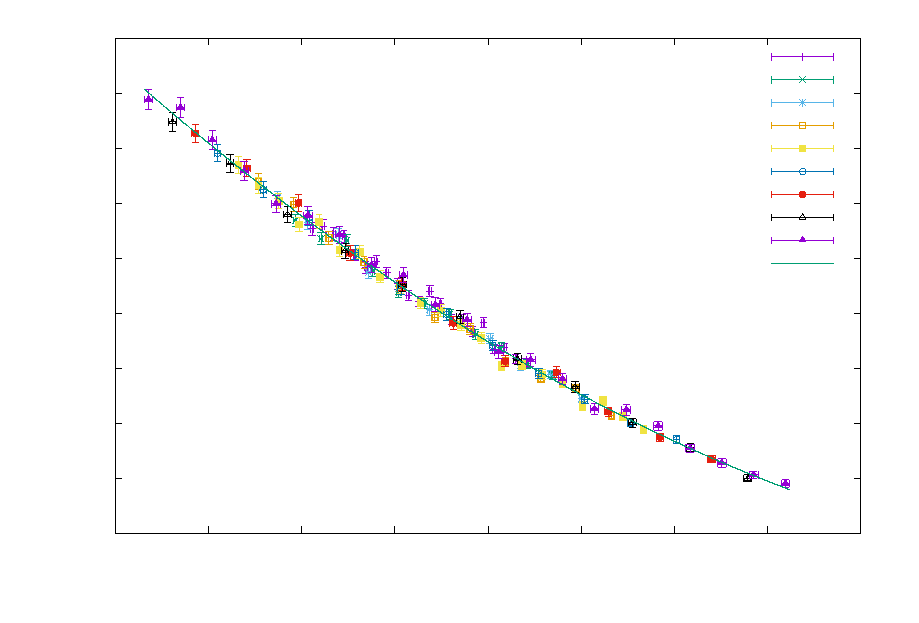
\includegraphics{./fin_size_scaling}}%
    \gplfronttext
  \end{picture}%
\endgroup

	\caption{test}
	\label{test4}
\end{figure}

\begin{figure}
	% GNUPLOT: LaTeX picture with Postscript
\begingroup
  % Encoding inside the plot.  In the header of your document, this encoding
  % should to defined, e.g., by using
  % \usepackage[latin1,<other encodings>]{inputenc}
  \inputencoding{latin1}%
  \makeatletter
  \providecommand\color[2][]{%
    \GenericError{(gnuplot) \space\space\space\@spaces}{%
      Package color not loaded in conjunction with
      terminal option `colourtext'%
    }{See the gnuplot documentation for explanation.%
    }{Either use 'blacktext' in gnuplot or load the package
      color.sty in LaTeX.}%
    \renewcommand\color[2][]{}%
  }%
  \providecommand\includegraphics[2][]{%
    \GenericError{(gnuplot) \space\space\space\@spaces}{%
      Package graphicx or graphics not loaded%
    }{See the gnuplot documentation for explanation.%
    }{The gnuplot epslatex terminal needs graphicx.sty or graphics.sty.}%
    \renewcommand\includegraphics[2][]{}%
  }%
  \providecommand\rotatebox[2]{#2}%
  \@ifundefined{ifGPcolor}{%
    \newif\ifGPcolor
    \GPcolortrue
  }{}%
  \@ifundefined{ifGPblacktext}{%
    \newif\ifGPblacktext
    \GPblacktextfalse
  }{}%
  % define a \g@addto@macro without @ in the name:
  \let\gplgaddtomacro\g@addto@macro
  % define empty templates for all commands taking text:
  \gdef\gplbacktext{}%
  \gdef\gplfronttext{}%
  \makeatother
  \ifGPblacktext
    % no textcolor at all
    \def\colorrgb#1{}%
    \def\colorgray#1{}%
  \else
    % gray or color?
    \ifGPcolor
      \def\colorrgb#1{\color[rgb]{#1}}%
      \def\colorgray#1{\color[gray]{#1}}%
      \expandafter\def\csname LTw\endcsname{\color{white}}%
      \expandafter\def\csname LTb\endcsname{\color{black}}%
      \expandafter\def\csname LTa\endcsname{\color{black}}%
      \expandafter\def\csname LT0\endcsname{\color[rgb]{1,0,0}}%
      \expandafter\def\csname LT1\endcsname{\color[rgb]{0,1,0}}%
      \expandafter\def\csname LT2\endcsname{\color[rgb]{0,0,1}}%
      \expandafter\def\csname LT3\endcsname{\color[rgb]{1,0,1}}%
      \expandafter\def\csname LT4\endcsname{\color[rgb]{0,1,1}}%
      \expandafter\def\csname LT5\endcsname{\color[rgb]{1,1,0}}%
      \expandafter\def\csname LT6\endcsname{\color[rgb]{0,0,0}}%
      \expandafter\def\csname LT7\endcsname{\color[rgb]{1,0.3,0}}%
      \expandafter\def\csname LT8\endcsname{\color[rgb]{0.5,0.5,0.5}}%
    \else
      % gray
      \def\colorrgb#1{\color{black}}%
      \def\colorgray#1{\color[gray]{#1}}%
      \expandafter\def\csname LTw\endcsname{\color{white}}%
      \expandafter\def\csname LTb\endcsname{\color{black}}%
      \expandafter\def\csname LTa\endcsname{\color{black}}%
      \expandafter\def\csname LT0\endcsname{\color{black}}%
      \expandafter\def\csname LT1\endcsname{\color{black}}%
      \expandafter\def\csname LT2\endcsname{\color{black}}%
      \expandafter\def\csname LT3\endcsname{\color{black}}%
      \expandafter\def\csname LT4\endcsname{\color{black}}%
      \expandafter\def\csname LT5\endcsname{\color{black}}%
      \expandafter\def\csname LT6\endcsname{\color{black}}%
      \expandafter\def\csname LT7\endcsname{\color{black}}%
      \expandafter\def\csname LT8\endcsname{\color{black}}%
    \fi
  \fi
    \setlength{\unitlength}{0.0500bp}%
    \ifx\gptboxheight\undefined%
      \newlength{\gptboxheight}%
      \newlength{\gptboxwidth}%
      \newsavebox{\gptboxtext}%
    \fi%
    \setlength{\fboxrule}{0.5pt}%
    \setlength{\fboxsep}{1pt}%
\begin{picture}(8502.00,5102.00)%
    \gplgaddtomacro\gplbacktext{%
      \csname LTb\endcsname%%
      \put(814,704){\makebox(0,0)[r]{\strut{}$1.2$}}%
      \put(814,1168){\makebox(0,0)[r]{\strut{}$1.3$}}%
      \put(814,1632){\makebox(0,0)[r]{\strut{}$1.4$}}%
      \put(814,2096){\makebox(0,0)[r]{\strut{}$1.5$}}%
      \put(814,2560){\makebox(0,0)[r]{\strut{}$1.6$}}%
      \put(814,3025){\makebox(0,0)[r]{\strut{}$1.7$}}%
      \put(814,3489){\makebox(0,0)[r]{\strut{}$1.8$}}%
      \put(814,3953){\makebox(0,0)[r]{\strut{}$1.9$}}%
      \put(814,4417){\makebox(0,0)[r]{\strut{}$2$}}%
      \put(814,4881){\makebox(0,0)[r]{\strut{}$2.1$}}%
      \put(946,484){\makebox(0,0){\strut{}$-0.2$}}%
      \put(1741,484){\makebox(0,0){\strut{}$-0.15$}}%
      \put(2537,484){\makebox(0,0){\strut{}$-0.1$}}%
      \put(3332,484){\makebox(0,0){\strut{}$-0.05$}}%
      \put(4128,484){\makebox(0,0){\strut{}$0$}}%
      \put(4923,484){\makebox(0,0){\strut{}$0.05$}}%
      \put(5719,484){\makebox(0,0){\strut{}$0.1$}}%
      \put(6514,484){\makebox(0,0){\strut{}$0.15$}}%
      \put(7310,484){\makebox(0,0){\strut{}$0.2$}}%
      \put(8105,484){\makebox(0,0){\strut{}$0.25$}}%
    }%
    \gplgaddtomacro\gplfronttext{%
      \csname LTb\endcsname%%
      \put(198,2792){\rotatebox{-270}{\makebox(0,0){\strut{}$\frac{\langle L^4 \rangle}{\langle L^2 \rangle^2}$}}}%
      \put(4525,154){\makebox(0,0){\strut{}$\frac{\beta - \beta_c}{\beta_c}N_\sigma^{1/\nu}$}}%
      \csname LTb\endcsname%%
      \put(7118,4708){\makebox(0,0)[r]{\strut{}$N_\sigma =\  8$}}%
      \csname LTb\endcsname%%
      \put(7118,4488){\makebox(0,0)[r]{\strut{}$N_\sigma =\  9$}}%
      \csname LTb\endcsname%%
      \put(7118,4268){\makebox(0,0)[r]{\strut{}$N_\sigma = 10$}}%
      \csname LTb\endcsname%%
      \put(7118,4048){\makebox(0,0)[r]{\strut{}$N_\sigma = 11$}}%
      \csname LTb\endcsname%%
      \put(7118,3828){\makebox(0,0)[r]{\strut{}$N_\sigma = 12$}}%
      \csname LTb\endcsname%%
      \put(7118,3608){\makebox(0,0)[r]{\strut{}$N_\sigma = 13$}}%
      \csname LTb\endcsname%%
      \put(7118,3388){\makebox(0,0)[r]{\strut{}$N_\sigma = 14$}}%
      \csname LTb\endcsname%%
      \put(7118,3168){\makebox(0,0)[r]{\strut{}$N_\sigma = 15$}}%
      \csname LTb\endcsname%%
      \put(7118,2948){\makebox(0,0)[r]{\strut{}$N_\sigma = 16$}}%
      \csname LTb\endcsname%%
      \put(7118,2728){\makebox(0,0)[r]{\strut{}angepasste Gerade}}%
      \csname LTb\endcsname%%
      \put(1741,1168){\makebox(0,0)[l]{\strut{}$\beta_c=\num{2.2983+-0.0002}\qquad\nu=\num{0.72+-0.02}$}}%
      \put(1741,1632){\makebox(0,0)[l]{\strut{}reduziertes $\chi^2 = \num{2.53}$}}%
    }%
    \gplbacktext
    \put(0,0){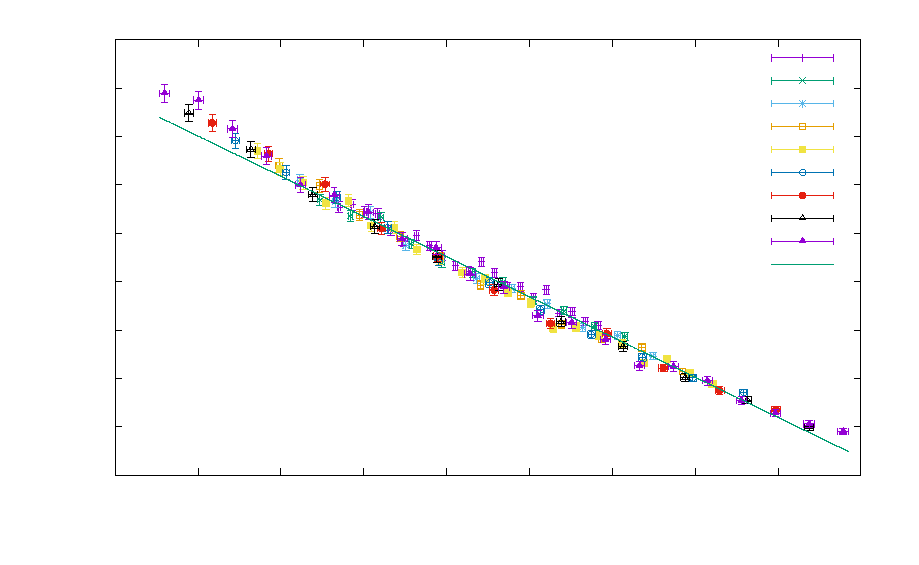
\includegraphics{./fin_size_scaling_straight}}%
    \gplfronttext
  \end{picture}%
\endgroup

	\caption{test}
	\label{t5est4}
\end{figure}

\begin{figure}
	% GNUPLOT: LaTeX picture with Postscript
\begingroup
  % Encoding inside the plot.  In the header of your document, this encoding
  % should to defined, e.g., by using
  % \usepackage[latin1,<other encodings>]{inputenc}
  \inputencoding{latin1}%
  \makeatletter
  \providecommand\color[2][]{%
    \GenericError{(gnuplot) \space\space\space\@spaces}{%
      Package color not loaded in conjunction with
      terminal option `colourtext'%
    }{See the gnuplot documentation for explanation.%
    }{Either use 'blacktext' in gnuplot or load the package
      color.sty in LaTeX.}%
    \renewcommand\color[2][]{}%
  }%
  \providecommand\includegraphics[2][]{%
    \GenericError{(gnuplot) \space\space\space\@spaces}{%
      Package graphicx or graphics not loaded%
    }{See the gnuplot documentation for explanation.%
    }{The gnuplot epslatex terminal needs graphicx.sty or graphics.sty.}%
    \renewcommand\includegraphics[2][]{}%
  }%
  \providecommand\rotatebox[2]{#2}%
  \@ifundefined{ifGPcolor}{%
    \newif\ifGPcolor
    \GPcolortrue
  }{}%
  \@ifundefined{ifGPblacktext}{%
    \newif\ifGPblacktext
    \GPblacktextfalse
  }{}%
  % define a \g@addto@macro without @ in the name:
  \let\gplgaddtomacro\g@addto@macro
  % define empty templates for all commands taking text:
  \gdef\gplbacktext{}%
  \gdef\gplfronttext{}%
  \makeatother
  \ifGPblacktext
    % no textcolor at all
    \def\colorrgb#1{}%
    \def\colorgray#1{}%
  \else
    % gray or color?
    \ifGPcolor
      \def\colorrgb#1{\color[rgb]{#1}}%
      \def\colorgray#1{\color[gray]{#1}}%
      \expandafter\def\csname LTw\endcsname{\color{white}}%
      \expandafter\def\csname LTb\endcsname{\color{black}}%
      \expandafter\def\csname LTa\endcsname{\color{black}}%
      \expandafter\def\csname LT0\endcsname{\color[rgb]{1,0,0}}%
      \expandafter\def\csname LT1\endcsname{\color[rgb]{0,1,0}}%
      \expandafter\def\csname LT2\endcsname{\color[rgb]{0,0,1}}%
      \expandafter\def\csname LT3\endcsname{\color[rgb]{1,0,1}}%
      \expandafter\def\csname LT4\endcsname{\color[rgb]{0,1,1}}%
      \expandafter\def\csname LT5\endcsname{\color[rgb]{1,1,0}}%
      \expandafter\def\csname LT6\endcsname{\color[rgb]{0,0,0}}%
      \expandafter\def\csname LT7\endcsname{\color[rgb]{1,0.3,0}}%
      \expandafter\def\csname LT8\endcsname{\color[rgb]{0.5,0.5,0.5}}%
    \else
      % gray
      \def\colorrgb#1{\color{black}}%
      \def\colorgray#1{\color[gray]{#1}}%
      \expandafter\def\csname LTw\endcsname{\color{white}}%
      \expandafter\def\csname LTb\endcsname{\color{black}}%
      \expandafter\def\csname LTa\endcsname{\color{black}}%
      \expandafter\def\csname LT0\endcsname{\color{black}}%
      \expandafter\def\csname LT1\endcsname{\color{black}}%
      \expandafter\def\csname LT2\endcsname{\color{black}}%
      \expandafter\def\csname LT3\endcsname{\color{black}}%
      \expandafter\def\csname LT4\endcsname{\color{black}}%
      \expandafter\def\csname LT5\endcsname{\color{black}}%
      \expandafter\def\csname LT6\endcsname{\color{black}}%
      \expandafter\def\csname LT7\endcsname{\color{black}}%
      \expandafter\def\csname LT8\endcsname{\color{black}}%
    \fi
  \fi
    \setlength{\unitlength}{0.0500bp}%
    \ifx\gptboxheight\undefined%
      \newlength{\gptboxheight}%
      \newlength{\gptboxwidth}%
      \newsavebox{\gptboxtext}%
    \fi%
    \setlength{\fboxrule}{0.5pt}%
    \setlength{\fboxsep}{1pt}%
\begin{picture}(8502.00,5102.00)%
    \gplgaddtomacro\gplbacktext{%
      \csname LTb\endcsname%%
      \put(946,704){\makebox(0,0)[r]{\strut{}$0.09$}}%
      \put(946,1226){\makebox(0,0)[r]{\strut{}$0.1$}}%
      \put(946,1748){\makebox(0,0)[r]{\strut{}$0.11$}}%
      \put(946,2270){\makebox(0,0)[r]{\strut{}$0.12$}}%
      \put(946,2792){\makebox(0,0)[r]{\strut{}$0.13$}}%
      \put(946,3315){\makebox(0,0)[r]{\strut{}$0.14$}}%
      \put(946,3837){\makebox(0,0)[r]{\strut{}$0.15$}}%
      \put(946,4359){\makebox(0,0)[r]{\strut{}$0.16$}}%
      \put(946,4881){\makebox(0,0)[r]{\strut{}$0.17$}}%
      \put(1397,484){\makebox(0,0){\strut{}$2.29$}}%
      \put(2994,484){\makebox(0,0){\strut{}$2.295$}}%
      \put(4591,484){\makebox(0,0){\strut{}$2.3$}}%
      \put(6189,484){\makebox(0,0){\strut{}$2.305$}}%
      \put(7786,484){\makebox(0,0){\strut{}$2.31$}}%
    }%
    \gplgaddtomacro\gplfronttext{%
      \csname LTb\endcsname%%
      \put(198,2792){\rotatebox{-270}{\makebox(0,0){\strut{}$\langle |L| \rangle$}}}%
      \put(4591,154){\makebox(0,0){\strut{}$\beta$}}%
      \csname LTb\endcsname%%
      \put(7118,4708){\makebox(0,0)[r]{\strut{}Nur Metropolis Updates: Daten}}%
      \csname LTb\endcsname%%
      \put(7118,4488){\makebox(0,0)[r]{\strut{}Metropolis und Overrelaxation Updates: Daten}}%
      \csname LTb\endcsname%%
      \put(7118,4268){\makebox(0,0)[r]{\strut{}Nur Metropolis Updates: Anpassung $\chi^2=\num{1.26}$}}%
      \csname LTb\endcsname%%
      \put(7118,4048){\makebox(0,0)[r]{\strut{}Metropolis und Overrelaxation Updates: Anpassung $\chi^2=\num{1.85}$}}%
      \csname LTb\endcsname%%
      \put(-777959,69102){\makebox(0,0)[l]{\strut{}reduziertes $\chi^2 = \num{2.53}$}}%
    }%
    \gplbacktext
    \put(0,0){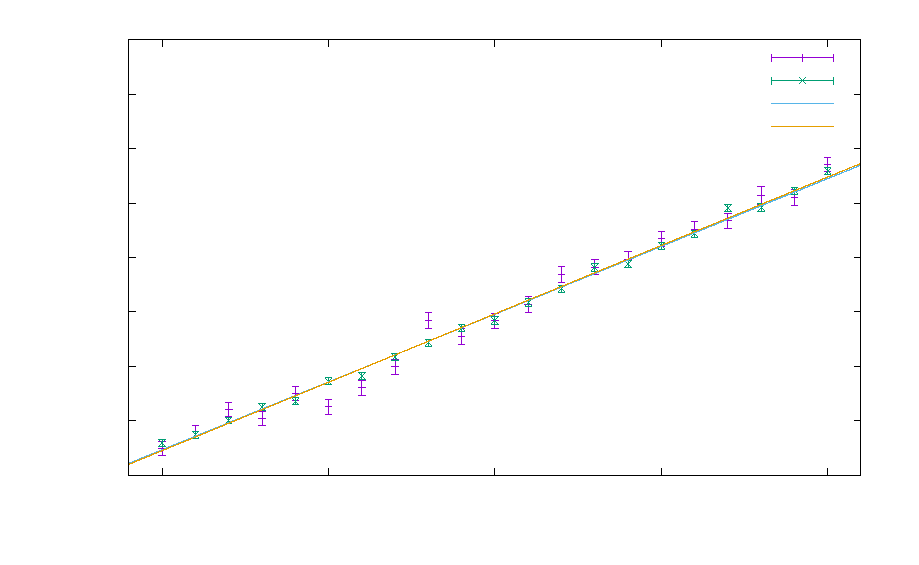
\includegraphics{overr_metropolis_comp}}%
    \gplfronttext
  \end{picture}%
\endgroup

	\caption{test}
	\label{tes7t4}
\end{figure}


\begin{figure}
	% GNUPLOT: LaTeX picture with Postscript
\begingroup
  % Encoding inside the plot.  In the header of your document, this encoding
  % should to defined, e.g., by using
  % \usepackage[latin1,<other encodings>]{inputenc}
  \inputencoding{latin1}%
  \makeatletter
  \providecommand\color[2][]{%
    \GenericError{(gnuplot) \space\space\space\@spaces}{%
      Package color not loaded in conjunction with
      terminal option `colourtext'%
    }{See the gnuplot documentation for explanation.%
    }{Either use 'blacktext' in gnuplot or load the package
      color.sty in LaTeX.}%
    \renewcommand\color[2][]{}%
  }%
  \providecommand\includegraphics[2][]{%
    \GenericError{(gnuplot) \space\space\space\@spaces}{%
      Package graphicx or graphics not loaded%
    }{See the gnuplot documentation for explanation.%
    }{The gnuplot epslatex terminal needs graphicx.sty or graphics.sty.}%
    \renewcommand\includegraphics[2][]{}%
  }%
  \providecommand\rotatebox[2]{#2}%
  \@ifundefined{ifGPcolor}{%
    \newif\ifGPcolor
    \GPcolortrue
  }{}%
  \@ifundefined{ifGPblacktext}{%
    \newif\ifGPblacktext
    \GPblacktextfalse
  }{}%
  % define a \g@addto@macro without @ in the name:
  \let\gplgaddtomacro\g@addto@macro
  % define empty templates for all commands taking text:
  \gdef\gplbacktext{}%
  \gdef\gplfronttext{}%
  \makeatother
  \ifGPblacktext
    % no textcolor at all
    \def\colorrgb#1{}%
    \def\colorgray#1{}%
  \else
    % gray or color?
    \ifGPcolor
      \def\colorrgb#1{\color[rgb]{#1}}%
      \def\colorgray#1{\color[gray]{#1}}%
      \expandafter\def\csname LTw\endcsname{\color{white}}%
      \expandafter\def\csname LTb\endcsname{\color{black}}%
      \expandafter\def\csname LTa\endcsname{\color{black}}%
      \expandafter\def\csname LT0\endcsname{\color[rgb]{1,0,0}}%
      \expandafter\def\csname LT1\endcsname{\color[rgb]{0,1,0}}%
      \expandafter\def\csname LT2\endcsname{\color[rgb]{0,0,1}}%
      \expandafter\def\csname LT3\endcsname{\color[rgb]{1,0,1}}%
      \expandafter\def\csname LT4\endcsname{\color[rgb]{0,1,1}}%
      \expandafter\def\csname LT5\endcsname{\color[rgb]{1,1,0}}%
      \expandafter\def\csname LT6\endcsname{\color[rgb]{0,0,0}}%
      \expandafter\def\csname LT7\endcsname{\color[rgb]{1,0.3,0}}%
      \expandafter\def\csname LT8\endcsname{\color[rgb]{0.5,0.5,0.5}}%
    \else
      % gray
      \def\colorrgb#1{\color{black}}%
      \def\colorgray#1{\color[gray]{#1}}%
      \expandafter\def\csname LTw\endcsname{\color{white}}%
      \expandafter\def\csname LTb\endcsname{\color{black}}%
      \expandafter\def\csname LTa\endcsname{\color{black}}%
      \expandafter\def\csname LT0\endcsname{\color{black}}%
      \expandafter\def\csname LT1\endcsname{\color{black}}%
      \expandafter\def\csname LT2\endcsname{\color{black}}%
      \expandafter\def\csname LT3\endcsname{\color{black}}%
      \expandafter\def\csname LT4\endcsname{\color{black}}%
      \expandafter\def\csname LT5\endcsname{\color{black}}%
      \expandafter\def\csname LT6\endcsname{\color{black}}%
      \expandafter\def\csname LT7\endcsname{\color{black}}%
      \expandafter\def\csname LT8\endcsname{\color{black}}%
    \fi
  \fi
    \setlength{\unitlength}{0.0500bp}%
    \ifx\gptboxheight\undefined%
      \newlength{\gptboxheight}%
      \newlength{\gptboxwidth}%
      \newsavebox{\gptboxtext}%
    \fi%
    \setlength{\fboxrule}{0.5pt}%
    \setlength{\fboxsep}{1pt}%
\begin{picture}(8502.00,5102.00)%
    \gplgaddtomacro\gplbacktext{%
      \csname LTb\endcsname%%
      \put(814,704){\makebox(0,0)[r]{\strut{}$0$}}%
      \put(814,1301){\makebox(0,0)[r]{\strut{}$0.1$}}%
      \put(814,1897){\makebox(0,0)[r]{\strut{}$0.2$}}%
      \put(814,2494){\makebox(0,0)[r]{\strut{}$0.3$}}%
      \put(814,3091){\makebox(0,0)[r]{\strut{}$0.4$}}%
      \put(814,3688){\makebox(0,0)[r]{\strut{}$0.5$}}%
      \put(814,4284){\makebox(0,0)[r]{\strut{}$0.6$}}%
      \put(814,4881){\makebox(0,0)[r]{\strut{}$0.7$}}%
      \put(1457,484){\makebox(0,0){\strut{}$2$}}%
      \put(2480,484){\makebox(0,0){\strut{}$3$}}%
      \put(3503,484){\makebox(0,0){\strut{}$4$}}%
      \put(4526,484){\makebox(0,0){\strut{}$5$}}%
      \put(5548,484){\makebox(0,0){\strut{}$6$}}%
      \put(6571,484){\makebox(0,0){\strut{}$7$}}%
      \put(7594,484){\makebox(0,0){\strut{}$8$}}%
    }%
    \gplgaddtomacro\gplfronttext{%
      \csname LTb\endcsname%%
      \put(198,2792){\rotatebox{-270}{\makebox(0,0){\strut{}$\langle |L| \rangle$}}}%
      \put(4525,154){\makebox(0,0){\strut{}$N_\tau$}}%
      \csname LTb\endcsname%%
      \put(-739,9058){\makebox(0,0)[l]{\strut{}reduziertes $\chi^2 = \num{2.53}$}}%
    }%
    \gplbacktext
    \put(0,0){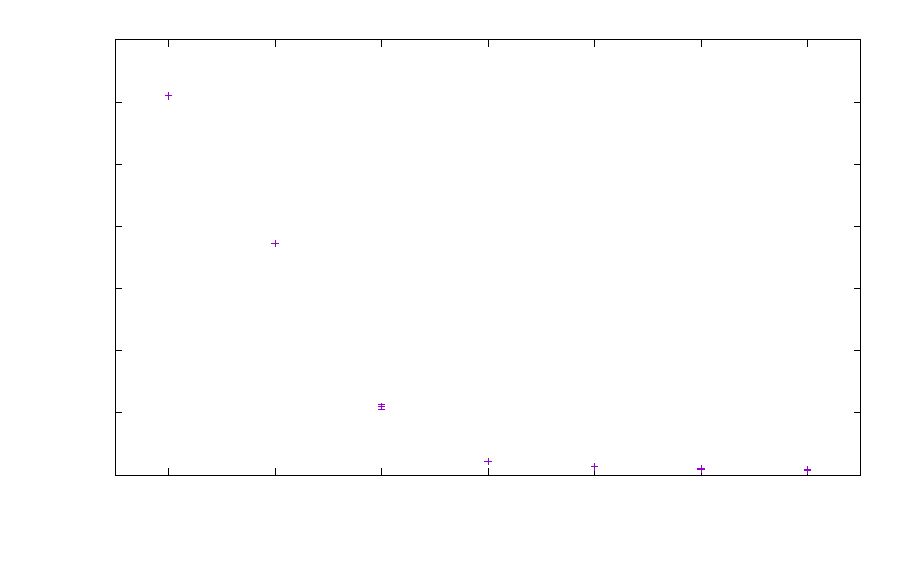
\includegraphics{temperature_scan_order}}%
    \gplfronttext
  \end{picture}%
\endgroup

	\caption{test}
	\label{t18est}
\end{figure}

\begin{figure}
	% GNUPLOT: LaTeX picture with Postscript
\begingroup
  % Encoding inside the plot.  In the header of your document, this encoding
  % should to defined, e.g., by using
  % \usepackage[latin1,<other encodings>]{inputenc}
  \inputencoding{latin1}%
  \makeatletter
  \providecommand\color[2][]{%
    \GenericError{(gnuplot) \space\space\space\@spaces}{%
      Package color not loaded in conjunction with
      terminal option `colourtext'%
    }{See the gnuplot documentation for explanation.%
    }{Either use 'blacktext' in gnuplot or load the package
      color.sty in LaTeX.}%
    \renewcommand\color[2][]{}%
  }%
  \providecommand\includegraphics[2][]{%
    \GenericError{(gnuplot) \space\space\space\@spaces}{%
      Package graphicx or graphics not loaded%
    }{See the gnuplot documentation for explanation.%
    }{The gnuplot epslatex terminal needs graphicx.sty or graphics.sty.}%
    \renewcommand\includegraphics[2][]{}%
  }%
  \providecommand\rotatebox[2]{#2}%
  \@ifundefined{ifGPcolor}{%
    \newif\ifGPcolor
    \GPcolortrue
  }{}%
  \@ifundefined{ifGPblacktext}{%
    \newif\ifGPblacktext
    \GPblacktextfalse
  }{}%
  % define a \g@addto@macro without @ in the name:
  \let\gplgaddtomacro\g@addto@macro
  % define empty templates for all commands taking text:
  \gdef\gplbacktext{}%
  \gdef\gplfronttext{}%
  \makeatother
  \ifGPblacktext
    % no textcolor at all
    \def\colorrgb#1{}%
    \def\colorgray#1{}%
  \else
    % gray or color?
    \ifGPcolor
      \def\colorrgb#1{\color[rgb]{#1}}%
      \def\colorgray#1{\color[gray]{#1}}%
      \expandafter\def\csname LTw\endcsname{\color{white}}%
      \expandafter\def\csname LTb\endcsname{\color{black}}%
      \expandafter\def\csname LTa\endcsname{\color{black}}%
      \expandafter\def\csname LT0\endcsname{\color[rgb]{1,0,0}}%
      \expandafter\def\csname LT1\endcsname{\color[rgb]{0,1,0}}%
      \expandafter\def\csname LT2\endcsname{\color[rgb]{0,0,1}}%
      \expandafter\def\csname LT3\endcsname{\color[rgb]{1,0,1}}%
      \expandafter\def\csname LT4\endcsname{\color[rgb]{0,1,1}}%
      \expandafter\def\csname LT5\endcsname{\color[rgb]{1,1,0}}%
      \expandafter\def\csname LT6\endcsname{\color[rgb]{0,0,0}}%
      \expandafter\def\csname LT7\endcsname{\color[rgb]{1,0.3,0}}%
      \expandafter\def\csname LT8\endcsname{\color[rgb]{0.5,0.5,0.5}}%
    \else
      % gray
      \def\colorrgb#1{\color{black}}%
      \def\colorgray#1{\color[gray]{#1}}%
      \expandafter\def\csname LTw\endcsname{\color{white}}%
      \expandafter\def\csname LTb\endcsname{\color{black}}%
      \expandafter\def\csname LTa\endcsname{\color{black}}%
      \expandafter\def\csname LT0\endcsname{\color{black}}%
      \expandafter\def\csname LT1\endcsname{\color{black}}%
      \expandafter\def\csname LT2\endcsname{\color{black}}%
      \expandafter\def\csname LT3\endcsname{\color{black}}%
      \expandafter\def\csname LT4\endcsname{\color{black}}%
      \expandafter\def\csname LT5\endcsname{\color{black}}%
      \expandafter\def\csname LT6\endcsname{\color{black}}%
      \expandafter\def\csname LT7\endcsname{\color{black}}%
      \expandafter\def\csname LT8\endcsname{\color{black}}%
    \fi
  \fi
    \setlength{\unitlength}{0.0500bp}%
    \ifx\gptboxheight\undefined%
      \newlength{\gptboxheight}%
      \newlength{\gptboxwidth}%
      \newsavebox{\gptboxtext}%
    \fi%
    \setlength{\fboxrule}{0.5pt}%
    \setlength{\fboxsep}{1pt}%
\begin{picture}(8502.00,5102.00)%
    \gplgaddtomacro\gplbacktext{%
      \csname LTb\endcsname%%
      \put(682,704){\makebox(0,0)[r]{\strut{}$0$}}%
      \put(682,1226){\makebox(0,0)[r]{\strut{}$5$}}%
      \put(682,1748){\makebox(0,0)[r]{\strut{}$10$}}%
      \put(682,2270){\makebox(0,0)[r]{\strut{}$15$}}%
      \put(682,2793){\makebox(0,0)[r]{\strut{}$20$}}%
      \put(682,3315){\makebox(0,0)[r]{\strut{}$25$}}%
      \put(682,3837){\makebox(0,0)[r]{\strut{}$30$}}%
      \put(682,4359){\makebox(0,0)[r]{\strut{}$35$}}%
      \put(682,4881){\makebox(0,0)[r]{\strut{}$40$}}%
      \put(1335,484){\makebox(0,0){\strut{}$2$}}%
      \put(2376,484){\makebox(0,0){\strut{}$3$}}%
      \put(3418,484){\makebox(0,0){\strut{}$4$}}%
      \put(4460,484){\makebox(0,0){\strut{}$5$}}%
      \put(5501,484){\makebox(0,0){\strut{}$6$}}%
      \put(6543,484){\makebox(0,0){\strut{}$7$}}%
      \put(7584,484){\makebox(0,0){\strut{}$8$}}%
    }%
    \gplgaddtomacro\gplfronttext{%
      \csname LTb\endcsname%%
      \put(198,2792){\rotatebox{-270}{\makebox(0,0){\strut{}$\tau_{\text{int},|L|}$}}}%
      \put(4459,154){\makebox(0,0){\strut{}$N_\tau$}}%
      \csname LTb\endcsname%%
      \put(-903,850){\makebox(0,0)[l]{\strut{}reduziertes $\chi^2 = \num{2.53}$}}%
    }%
    \gplbacktext
    \put(0,0){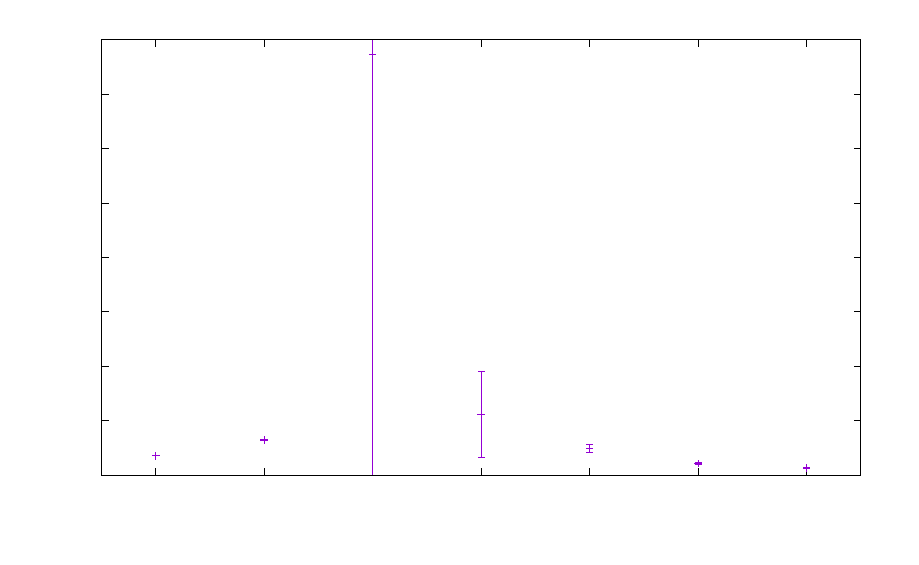
\includegraphics{temperature_scan_order_ctime}}%
    \gplfronttext
  \end{picture}%
\endgroup

	\caption{test}
	\label{te9st}
\end{figure}




\begin{figure}
	% GNUPLOT: LaTeX picture with Postscript
\begingroup
  % Encoding inside the plot.  In the header of your document, this encoding
  % should to defined, e.g., by using
  % \usepackage[latin1,<other encodings>]{inputenc}
  \inputencoding{latin1}%
  \makeatletter
  \providecommand\color[2][]{%
    \GenericError{(gnuplot) \space\space\space\@spaces}{%
      Package color not loaded in conjunction with
      terminal option `colourtext'%
    }{See the gnuplot documentation for explanation.%
    }{Either use 'blacktext' in gnuplot or load the package
      color.sty in LaTeX.}%
    \renewcommand\color[2][]{}%
  }%
  \providecommand\includegraphics[2][]{%
    \GenericError{(gnuplot) \space\space\space\@spaces}{%
      Package graphicx or graphics not loaded%
    }{See the gnuplot documentation for explanation.%
    }{The gnuplot epslatex terminal needs graphicx.sty or graphics.sty.}%
    \renewcommand\includegraphics[2][]{}%
  }%
  \providecommand\rotatebox[2]{#2}%
  \@ifundefined{ifGPcolor}{%
    \newif\ifGPcolor
    \GPcolortrue
  }{}%
  \@ifundefined{ifGPblacktext}{%
    \newif\ifGPblacktext
    \GPblacktextfalse
  }{}%
  % define a \g@addto@macro without @ in the name:
  \let\gplgaddtomacro\g@addto@macro
  % define empty templates for all commands taking text:
  \gdef\gplbacktext{}%
  \gdef\gplfronttext{}%
  \makeatother
  \ifGPblacktext
    % no textcolor at all
    \def\colorrgb#1{}%
    \def\colorgray#1{}%
  \else
    % gray or color?
    \ifGPcolor
      \def\colorrgb#1{\color[rgb]{#1}}%
      \def\colorgray#1{\color[gray]{#1}}%
      \expandafter\def\csname LTw\endcsname{\color{white}}%
      \expandafter\def\csname LTb\endcsname{\color{black}}%
      \expandafter\def\csname LTa\endcsname{\color{black}}%
      \expandafter\def\csname LT0\endcsname{\color[rgb]{1,0,0}}%
      \expandafter\def\csname LT1\endcsname{\color[rgb]{0,1,0}}%
      \expandafter\def\csname LT2\endcsname{\color[rgb]{0,0,1}}%
      \expandafter\def\csname LT3\endcsname{\color[rgb]{1,0,1}}%
      \expandafter\def\csname LT4\endcsname{\color[rgb]{0,1,1}}%
      \expandafter\def\csname LT5\endcsname{\color[rgb]{1,1,0}}%
      \expandafter\def\csname LT6\endcsname{\color[rgb]{0,0,0}}%
      \expandafter\def\csname LT7\endcsname{\color[rgb]{1,0.3,0}}%
      \expandafter\def\csname LT8\endcsname{\color[rgb]{0.5,0.5,0.5}}%
    \else
      % gray
      \def\colorrgb#1{\color{black}}%
      \def\colorgray#1{\color[gray]{#1}}%
      \expandafter\def\csname LTw\endcsname{\color{white}}%
      \expandafter\def\csname LTb\endcsname{\color{black}}%
      \expandafter\def\csname LTa\endcsname{\color{black}}%
      \expandafter\def\csname LT0\endcsname{\color{black}}%
      \expandafter\def\csname LT1\endcsname{\color{black}}%
      \expandafter\def\csname LT2\endcsname{\color{black}}%
      \expandafter\def\csname LT3\endcsname{\color{black}}%
      \expandafter\def\csname LT4\endcsname{\color{black}}%
      \expandafter\def\csname LT5\endcsname{\color{black}}%
      \expandafter\def\csname LT6\endcsname{\color{black}}%
      \expandafter\def\csname LT7\endcsname{\color{black}}%
      \expandafter\def\csname LT8\endcsname{\color{black}}%
    \fi
  \fi
    \setlength{\unitlength}{0.0500bp}%
    \ifx\gptboxheight\undefined%
      \newlength{\gptboxheight}%
      \newlength{\gptboxwidth}%
      \newsavebox{\gptboxtext}%
    \fi%
    \setlength{\fboxrule}{0.5pt}%
    \setlength{\fboxsep}{1pt}%
\begin{picture}(8502.00,5668.00)%
    \gplgaddtomacro\gplbacktext{%
      \csname LTb\endcsname%%
      \put(946,704){\makebox(0,0)[r]{\strut{}$0.07$}}%
      \put(946,1382){\makebox(0,0)[r]{\strut{}$0.08$}}%
      \put(946,2059){\makebox(0,0)[r]{\strut{}$0.09$}}%
      \put(946,2737){\makebox(0,0)[r]{\strut{}$0.1$}}%
      \put(946,3414){\makebox(0,0)[r]{\strut{}$0.11$}}%
      \put(946,4092){\makebox(0,0)[r]{\strut{}$0.12$}}%
      \put(946,4769){\makebox(0,0)[r]{\strut{}$0.13$}}%
      \put(946,5447){\makebox(0,0)[r]{\strut{}$0.14$}}%
      \put(1078,484){\makebox(0,0){\strut{}$2.29$}}%
      \put(2835,484){\makebox(0,0){\strut{}$2.295$}}%
      \put(4591,484){\makebox(0,0){\strut{}$2.3$}}%
      \put(6348,484){\makebox(0,0){\strut{}$2.305$}}%
      \put(8105,484){\makebox(0,0){\strut{}$2.31$}}%
    }%
    \gplgaddtomacro\gplfronttext{%
      \csname LTb\endcsname%%
      \put(198,3075){\rotatebox{-270}{\makebox(0,0){\strut{}$langle |L| 
angle$}}}%
      \put(4591,154){\makebox(0,0){\strut{}$beta$}}%
      \csname LTb\endcsname%%
      \put(-891349,84045){\makebox(0,0)[l]{\strut{}$\beta_c=\num{2.2977+-0.0002}$, $\nu=\num{0.64+-0.02}$, reduced $\chi^2 = \num{1.05}$}}%
    }%
    \gplbacktext
    \put(0,0){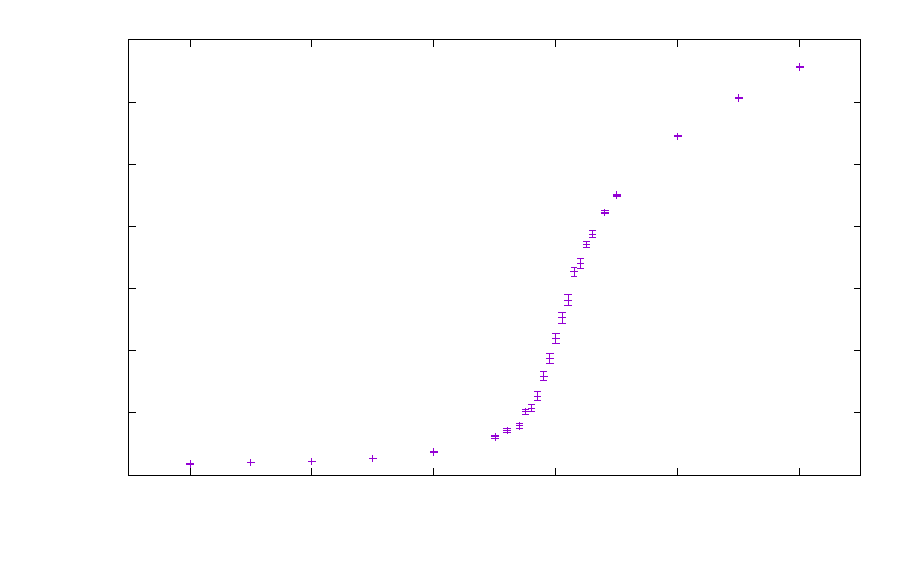
\includegraphics{beta_scan_order}}%
    \gplfronttext
  \end{picture}%
\endgroup

	\caption{test}
	\label{t1est}
\end{figure}

\begin{figure}
	% GNUPLOT: LaTeX picture with Postscript
\begingroup
  % Encoding inside the plot.  In the header of your document, this encoding
  % should to defined, e.g., by using
  % \usepackage[latin1,<other encodings>]{inputenc}
  \inputencoding{latin1}%
  \makeatletter
  \providecommand\color[2][]{%
    \GenericError{(gnuplot) \space\space\space\@spaces}{%
      Package color not loaded in conjunction with
      terminal option `colourtext'%
    }{See the gnuplot documentation for explanation.%
    }{Either use 'blacktext' in gnuplot or load the package
      color.sty in LaTeX.}%
    \renewcommand\color[2][]{}%
  }%
  \providecommand\includegraphics[2][]{%
    \GenericError{(gnuplot) \space\space\space\@spaces}{%
      Package graphicx or graphics not loaded%
    }{See the gnuplot documentation for explanation.%
    }{The gnuplot epslatex terminal needs graphicx.sty or graphics.sty.}%
    \renewcommand\includegraphics[2][]{}%
  }%
  \providecommand\rotatebox[2]{#2}%
  \@ifundefined{ifGPcolor}{%
    \newif\ifGPcolor
    \GPcolortrue
  }{}%
  \@ifundefined{ifGPblacktext}{%
    \newif\ifGPblacktext
    \GPblacktextfalse
  }{}%
  % define a \g@addto@macro without @ in the name:
  \let\gplgaddtomacro\g@addto@macro
  % define empty templates for all commands taking text:
  \gdef\gplbacktext{}%
  \gdef\gplfronttext{}%
  \makeatother
  \ifGPblacktext
    % no textcolor at all
    \def\colorrgb#1{}%
    \def\colorgray#1{}%
  \else
    % gray or color?
    \ifGPcolor
      \def\colorrgb#1{\color[rgb]{#1}}%
      \def\colorgray#1{\color[gray]{#1}}%
      \expandafter\def\csname LTw\endcsname{\color{white}}%
      \expandafter\def\csname LTb\endcsname{\color{black}}%
      \expandafter\def\csname LTa\endcsname{\color{black}}%
      \expandafter\def\csname LT0\endcsname{\color[rgb]{1,0,0}}%
      \expandafter\def\csname LT1\endcsname{\color[rgb]{0,1,0}}%
      \expandafter\def\csname LT2\endcsname{\color[rgb]{0,0,1}}%
      \expandafter\def\csname LT3\endcsname{\color[rgb]{1,0,1}}%
      \expandafter\def\csname LT4\endcsname{\color[rgb]{0,1,1}}%
      \expandafter\def\csname LT5\endcsname{\color[rgb]{1,1,0}}%
      \expandafter\def\csname LT6\endcsname{\color[rgb]{0,0,0}}%
      \expandafter\def\csname LT7\endcsname{\color[rgb]{1,0.3,0}}%
      \expandafter\def\csname LT8\endcsname{\color[rgb]{0.5,0.5,0.5}}%
    \else
      % gray
      \def\colorrgb#1{\color{black}}%
      \def\colorgray#1{\color[gray]{#1}}%
      \expandafter\def\csname LTw\endcsname{\color{white}}%
      \expandafter\def\csname LTb\endcsname{\color{black}}%
      \expandafter\def\csname LTa\endcsname{\color{black}}%
      \expandafter\def\csname LT0\endcsname{\color{black}}%
      \expandafter\def\csname LT1\endcsname{\color{black}}%
      \expandafter\def\csname LT2\endcsname{\color{black}}%
      \expandafter\def\csname LT3\endcsname{\color{black}}%
      \expandafter\def\csname LT4\endcsname{\color{black}}%
      \expandafter\def\csname LT5\endcsname{\color{black}}%
      \expandafter\def\csname LT6\endcsname{\color{black}}%
      \expandafter\def\csname LT7\endcsname{\color{black}}%
      \expandafter\def\csname LT8\endcsname{\color{black}}%
    \fi
  \fi
    \setlength{\unitlength}{0.0500bp}%
    \ifx\gptboxheight\undefined%
      \newlength{\gptboxheight}%
      \newlength{\gptboxwidth}%
      \newsavebox{\gptboxtext}%
    \fi%
    \setlength{\fboxrule}{0.5pt}%
    \setlength{\fboxsep}{1pt}%
\begin{picture}(8502.00,5668.00)%
    \gplgaddtomacro\gplbacktext{%
      \csname LTb\endcsname%%
      \put(946,704){\makebox(0,0)[r]{\strut{}$0.75$}}%
      \put(946,1297){\makebox(0,0)[r]{\strut{}$0.8$}}%
      \put(946,1890){\makebox(0,0)[r]{\strut{}$0.85$}}%
      \put(946,2483){\makebox(0,0)[r]{\strut{}$0.9$}}%
      \put(946,3076){\makebox(0,0)[r]{\strut{}$0.95$}}%
      \put(946,3668){\makebox(0,0)[r]{\strut{}$1$}}%
      \put(946,4261){\makebox(0,0)[r]{\strut{}$1.05$}}%
      \put(946,4854){\makebox(0,0)[r]{\strut{}$1.1$}}%
      \put(946,5447){\makebox(0,0)[r]{\strut{}$1.15$}}%
      \put(1078,484){\makebox(0,0){\strut{}$2.29$}}%
      \put(2835,484){\makebox(0,0){\strut{}$2.295$}}%
      \put(4591,484){\makebox(0,0){\strut{}$2.3$}}%
      \put(6348,484){\makebox(0,0){\strut{}$2.305$}}%
      \put(8105,484){\makebox(0,0){\strut{}$2.31$}}%
    }%
    \gplgaddtomacro\gplfronttext{%
      \csname LTb\endcsname%%
      \put(198,3075){\rotatebox{-270}{\makebox(0,0){\strut{}$	au_{	ext{int},|L|}$}}}%
      \put(4591,154){\makebox(0,0){\strut{}$beta$}}%
      \csname LTb\endcsname%%
      \put(-891349,7226){\makebox(0,0)[l]{\strut{}$\beta_c=\num{2.2977+-0.0002}$, $\nu=\num{0.64+-0.02}$, reduced $\chi^2 = \num{1.05}$}}%
    }%
    \gplbacktext
    \put(0,0){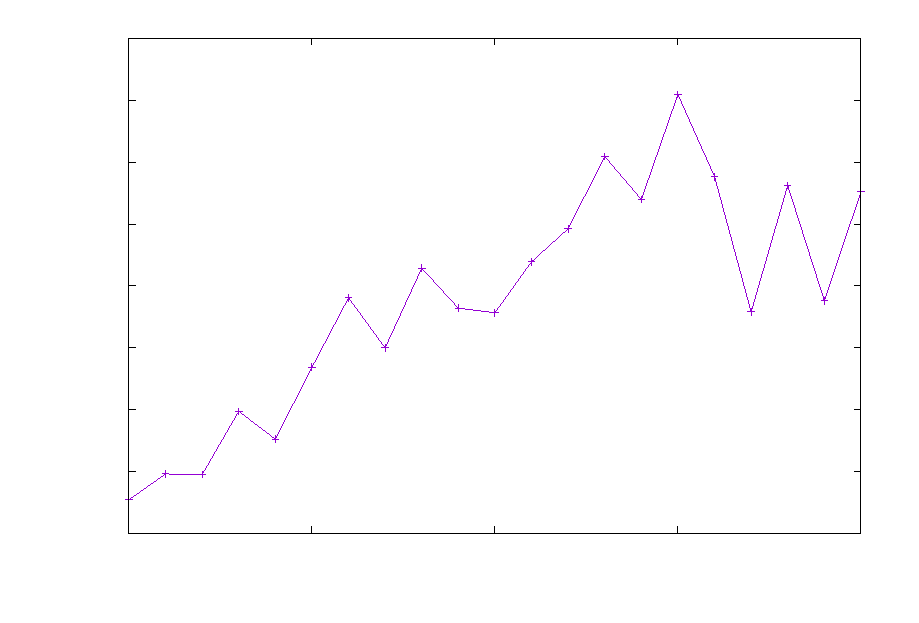
\includegraphics{beta_scan_order_ctime}}%
    \gplfronttext
  \end{picture}%
\endgroup

	\caption{test}
	\label{test}
\end{figure}

\begin{figure}
	\centering
	\begin{tikzpicture}[scale=3]
	\draw [<->] (-0.5,0.25) -- (-0.5,0.5) -- (-0.25,0.5);
	\path (-0.5,0.25) node[align=center, right] {$\nu$} (-0.25,0.5) node[align=center, above] {$\mu$};
	\draw [-latex, ultra thick] (0.05,0) --node[align=center, below]{$U_\mu^{\mathop{\vphantom{\dag}}}(x)$} (0.95,0);
	\draw [latex-, ultra thick] (1.05,0) --node[align=center, below]{$U_\mu^\dag(x+\hat{\mu})$} (1.95,0);
	\draw [ultra thin, dashed] (-0.5,0) -- (-0.05,0);
	\draw [ultra thin, dashed] (2.05,0) -- (2.5,0);
	\draw [ultra thin, dashed] (0,-0.5) -- (0,-0.05);
	\draw [ultra thin, dashed] (0,0.05) -- (0,0.5);
	\draw [ultra thin, dashed] (1,-0.5) -- (1,-0.05);
	\draw [ultra thin, dashed] (1,0.18) -- (1,0.5);
	\draw [ultra thin, dashed] (2,-0.5) -- (2,-0.05);
	\draw [ultra thin, dashed] (2,0.05) -- (2,0.5);
	\filldraw (0,0) circle (0.5pt) node[align=center, above left]{$x$};
	\filldraw (1,0) circle (0.5pt) node[align=center, above]{$x + \hat{\mu}$};
	\filldraw (2,0) circle (0.5pt) node[align=center, above right]{$x + 2\hat{\mu}$};
	\end{tikzpicture}
\end{figure}

\begin{figure}
	\centering
	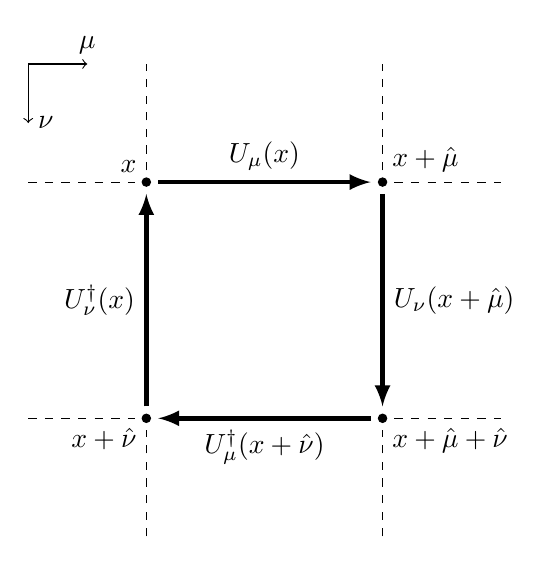
\begin{tikzpicture}[scale=3]
	\draw [<->] (-0.5,0.25) -- (-0.5,0.5) -- (-0.25,0.5);
	\path (-0.5,0.25) node[align=center, right] {$\nu$} (-0.25,0.5) node[align=center, above] {$\mu$};
	\draw [-latex, ultra thick] (0.05,0) --node[align=center, above]{$U_\mu(x)$} (0.95,0);
	\draw [-latex, ultra thick] (1,-0.05) --node[align=center, right]{$U_\nu(x+\hat{\mu})$} (1,-0.95);
	\draw [-latex, ultra thick] (0.95,-1) --node[align=center, below]{$U_\mu^\dag(x+\hat{\nu})$} (0.05,-1);
	\draw [-latex, ultra thick] (0,-0.95) --node[align=center, left]{$U_\nu^\dag(x)$} (0,-0.05);
	\draw [ultra thin, dashed] (-0.5,0) -- (-0.05,0);
	\draw [ultra thin, dashed] (1.05,0) -- (1.5,0);
	\draw [ultra thin, dashed] (-0.5,-1) -- (-0.05,-1);
	\draw [ultra thin, dashed] (1.05,-1) -- (1.5,-1);
	\draw [ultra thin, dashed] (0,-1.5) -- (0,-1.05);
	\draw [ultra thin, dashed] (0,0.05) -- (0,0.5);
	\draw [ultra thin, dashed] (1,0.05) -- (1,0.5);
	\draw [ultra thin, dashed] (1,-1.5) -- (1,-1.05);
	\filldraw (0,0) circle (0.5pt) node[align=center, above left]{$x$};
	\filldraw (1,0) circle (0.5pt) node[align=center, above right]{$x + \hat{\mu}$};
	\filldraw (1,-1) circle (0.5pt) node[align=center, below right]{$x + \hat{\mu} + \hat{\nu}$};
	\filldraw (0,-1) circle (0.5pt) node[align=center, below left]{$x + \hat{\nu}$};
	\end{tikzpicture}
\end{figure}

\begin{figure}
	\centering
	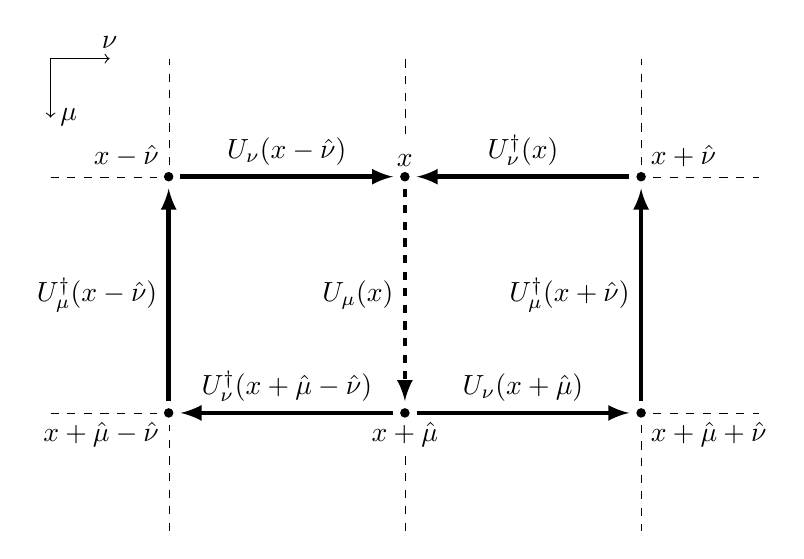
\begin{tikzpicture}[scale=3]
	\draw [<->] (-0.5,0.25) -- (-0.5,0.5) -- (-0.25,0.5);
	\path (-0.5,0.25) node[align=center, right] {$\mu$} (-0.25,0.5) node[align=center, above] {$\nu$};
	\draw [-latex, ultra thick] (0.05,0) --node[align=center, above]{$U_\nu(x-\hat{\nu})$} (0.95,0);
	\draw [latex-, ultra thick] (1.05,0) --node[align=center, above]{$U_\nu^\dag(x)$} (1.95,0);
	\draw [-latex, ultra thick, dashed] (1,-0.05) -- (1,-0.5) node[align=center, left] {$U_\mu(x)$} -- (1,-0.95);
	\draw [-latex, ultra thick] (0.95,-1) --node[align=center, above]{$U_\nu^\dag(x+\hat{\mu}-\hat{\nu})$} (0.05,-1);
	\draw [latex-, ultra thick] (1.95,-1) --node[align=center, above]{$U_\nu(x+\hat{\mu})$} (1.05,-1);
	\draw [-latex, ultra thick] (0,-0.95) --node[align=center, left]{$U_\mu^\dag(x-\hat{\nu})$} (0,-0.05);
	\draw [-latex, ultra thick] (2,-0.95) --node[align=center, left]{$U_\mu^\dag(x+\hat{\nu})$} (2,-0.05);
	\draw [ultra thin, dashed] (-0.5,0) -- (-0.05,0);
	\draw [ultra thin, dashed] (-0.5,-1) -- (-0.05,-1);
	\draw [ultra thin, dashed] (0,-1.5) -- (0,-1.05);
	\draw [ultra thin, dashed] (0,0.05) -- (0,0.5);
	\draw [ultra thin, dashed] (1,0.18) -- (1,0.5);
	\draw [ultra thin, dashed] (1,-1.5) -- (1,-1.18);
	\draw [ultra thin, dashed] (2.05,0) -- (2.5,0);
	\draw [ultra thin, dashed] (2,0.05) -- (2,0.5);
	\draw [ultra thin, dashed] (2.05,-1) -- (2.5,-1);
	\draw [ultra thin, dashed] (2,-1.05) -- (2,-1.5);
	\filldraw (0,0) circle (0.5pt) node[align=center, above left]{$x - \hat{\nu}$};
	\filldraw (1,0) circle (0.5pt) node[align=center, above]{$x$};
	\filldraw (1,-1) circle (0.5pt) node[align=center, below]{$x + \hat{\mu}$};
	\filldraw (0,-1) circle (0.5pt) node[align=center, below left]{$x + \hat{\mu} - \hat{\nu}$};
	\filldraw (2,0) circle (0.5pt) node[align=center, above right]{$x + \hat{\nu}$};
	\filldraw (2,-1) circle (0.5pt) node[align=center, below right]{$x + \hat{\mu} + \hat{\nu}$};
	\end{tikzpicture}
\end{figure}


\end{document}
